% Template: Fabian Wenzelmann, 2019
\documentclass{beamer}

\usepackage[utf8]{inputenc}
\usepackage[english]{babel} % use ngerman here for german text
\usepackage[T1]{fontenc}
\usepackage{mathtools}
\usepackage{amssymb}
\usepackage{lmodern}
\usepackage[protrusion=true,expansion=true,kerning]{microtype}
\usepackage{graphicx}
\usepackage{hyperref}
\usepackage{mdframed}
\usepackage{amsrefs}

\usepackage{caption}
\usepackage{subcaption}
\usepackage{float}

\usetheme{CambridgeUS}
\usecolortheme{dolphin}


% einige Abkuerzungen
\newcommand{\C}{\mathbb{C}} % komplexe
\newcommand{\K}{\mathbb{K}} % komplexe
\newcommand{\R}{\mathbb{R}} % reelle
\newcommand{\Q}{\mathbb{Q}} % rationale
\newcommand{\Z}{\mathbb{Z}} % ganze
\newcommand{\N}{\mathbb{N}} % natuerliche
\newcommand{\E}{\mathbb{E}} % Erwartungswert
\newcommand{\F}{\mathcal{F}} 
\newcommand{\G}{\mathcal{G}} 

\makeatletter
\newcommand{\vast}{\bBigg@{3}}
\newcommand{\Vast}{\bBigg@{5}}
\makeatother


\title[Koltchinskii \& Panchenko]{'Empirical margin distributions and bounding the generalization error of combined classifiers' \\ - Vladimir Koltchinskii \& Dimitry Panchenko}
\subtitle{Statsitcal Learning Seminar 4. Vortrag}

% For short you could for example use the last name only, it's optional as is
% the short title
\author[Statistical Learning Seminar]{Ben Deitmar}

% Can be set, for students usually not required
%\institute{}

\date{09.06.2020}

% removes the navigation symbols
% often they don't work and I find them rather annoying
\beamertemplatenavigationsymbolsempty{}

% You can have a logo to appear on all slides
 \logo{
\includegraphics[height=1cm]{Bilder/logo}}

% If you want that at the beginning of each section the table of contents
% is shown, I don't like it for short presentations
%\AtBeginSection[]
%{
%  \begin{frame}
%    \frametitle{Table of Contents}
%    \tableofcontents[currentsection]
%  \end{frame}
%}

%\tableofcontents

\begin{document}
	
	\begin{frame}
		\titlepage
	\end{frame}
	
	% TOC if you want it
	\begin{frame}
		\frametitle{Gliederung}
		\begin{itemize}
			\item Einführung Empirische Prozesse
			\item Rademacher-Komplexität
			\item L\'evi-Abstand
			\item Aussagen des Artikels
			\item Anwendungen
			\item Vergleich
		\end{itemize}
	\end{frame}


	\section{Empirische Prozesse}
	
	\begin{frame}
		\frametitle{Glivenko-Cantelli-Klassen}
		\begin{itemize}
			\item $P$ Verteilung auf $[0,1]\times\{-1,1\}$
			\item $\F \subset L^1(P)$\\
			d.h. $\F \subset \{ f : [0,1] \times \{-1,1\} \rightarrow \R \, mb. \mid \E_P[|f(X,Y)|]<\infty \}$
			\item $((X_1,Y_1),...,(X_n,Y_n)) \sim P^{\otimes n} : \ \ \hat{P}_n := \frac{1}{n} \sum\limits_{i=1}^n \delta_{(X_i,Y_i)}$
		\end{itemize}
		\hfill\break
		Definition:\\
		$\F$ ist $P$-\textbf{Glivenko-Cantelli-Klasse} $\Leftrightarrow \ \sup\limits_{f \in \F} \left| \hat{P}_n(f) - P(f) \right| \xrightarrow{n \rightarrow \infty}_{fs.} 0$
		\hfill\break
		\hfill\break
		\pause
		Problem: $\sup\limits_{f \in \F} \left| \hat{P}_n(f) - P(f) \right|$ nicht immer messbar.\\
		Kann man mit zusätzlichen Anforderungen an $\F$ beheben.\\ (siehe \cite{DudleyUCLT} Sektion 5.3)
	\end{frame}

	\begin{frame}
		\frametitle{Glivenko-Cantelli-Klassen}
		\begin{mdframed}
			\textbf{Starkes Gesetz der großen Zahlen:}\\
			$(X_1,Y_1),(X_2,Y_2),...uiv. \sim P$\\
			$ \ \Rightarrow \hat{P}_n(f) - P(f) = \frac{1}{n}\sum\limits_{i=1}^n f(X_i,Y_i)-\E_P[f] \xrightarrow{n \rightarrow \infty}_{fs.} 0$
		\end{mdframed}
		$ \ \ \ \Rightarrow \{f\}$ ist $P$-GC.
		\hfill\break
		\begin{mdframed}
			\textbf{Satz von Glivenko-Cantelli:}\\
			$\forall \widetilde{f} \in L^1(P) : \ \sup\limits_{z \in \R} |\hat{P}_n(\widetilde{f} \leq z)- P(\widetilde{f} \leq z)| \xrightarrow{n \rightarrow \infty}_{fs.} 0$
		\end{mdframed}
		$ \ \ \ \Rightarrow $ Für $\widetilde{f} \in L^1(P)$ ist $\{ 1_{\widetilde{f} \leq z} \mid z \in \R \}$ $P$-GC.
	\end{frame}
	
	\begin{frame}
		\frametitle{Donsker-Klassen}
		Definition:\\
		$\F \subset L^2(P)$ ist $P$-\textbf{Donsker-Klasse}\\
		$ \ \ \ \ \ \ \ \ \ \ \ \ \ \ \ \Leftrightarrow \ \exists G_P \text{ Prozess auf } \F : \ \sqrt{n}\big( \hat{P}_n(f)-P(f) \big)_{f \in \F} \xrightarrow{n \rightarrow \infty}_{\mathcal{L}} G_P$
		\hfill\break
		\hfill\break
		D.h. $\forall H \in C_b(\ell^\infty(\F)) :$\\
		$ \ \ \ \ \ \ \ \ \ \ \ \E\left[ H\left(\sqrt{n}\big( \hat{P}_n(f)-P(f) \big)_{f \in \F}\right) \right] \xrightarrow{n \rightarrow \infty} \E[H\left(G_P\right)]$
		\pause
		\begin{mdframed}
			\textbf{Zentraler Grenzwertsatz:}\\
			$\forall f \in L^2(P) :$\\
			$\sqrt{n}\big( \hat{P}_n(f)-P(f) \big) = \frac{1}{\sqrt{n}} \sum\limits_{i=1}^n f(X_i,Y_i)-\E_P[f] \xrightarrow{n \rightarrow \infty}_{\mathcal{L}} N(0,\sigma^2)$
		\end{mdframed}
		$ \ \ \ \Rightarrow \{f\}$ ist $P$-Donsker
	\end{frame}
	
	\begin{frame}
		\frametitle{Donsker-Klassen (Eigenschaften)}
		\begin{itemize}
			\item $\F$ $P$-Donsker und $\G \subset \F$ $ \ \Rightarrow \ \G$ $P$-Donsker
			\item $\F , \G$ $P$-Donsker $ \ \Rightarrow \ \F \cup \G$ $P$-Donsker
			\item $\F$ $P$-Donsker $ \ \Rightarrow \ co(\F)$ $P$-Donsker
			\item $\F$ $P$-Donsker $ \ \Rightarrow \ \E\left[ \sup\limits_{f \in \F} \left| \hat{P}_n(f) - P(f) \right| \right] \leq \frac{C}{\sqrt{n}}$
		\end{itemize}
		\pause
		\begin{mdframed}
			\textbf{Universelle Donsker-Klassen} (Dudley, 1992):\\
			$\forall M > 0 \ \forall P $ Verteilung auf $\R : \ E_M$ ist $P$-Donsker-Klasse\\
			für $E_M = \{f : \R \rightarrow \R \mid M \geq ||f||_{TV} \}$.\\
			\\
			(vgl. \cite{DudleyUCLT} Seite 329)
		\end{mdframed}
	\end{frame}
	
	\begin{frame}
		\frametitle{Lemma 1.4 Algorithmus-Risiko bei Donsker-Klassen}
		Für $y \in \{-1,1\}$:
		\begin{itemize}
			\item $P_y(A) := P_{X \mid Y=y}(A) = P(X \in A \mid Y=y)$ Verteilung auf $[0,1]$
			\item $L : \R \times \{-1,1\} \rightarrow [0,\infty]$ Verlustfunktion
			\item Funktionenfamilie $(f_\alpha)_{\alpha \in \Lambda}$
			\item $\F_y := \{ x \mapsto L(f_\alpha(x),y) \mid \alpha \in \Lambda \} \subset L^2(P_y)$
			\item falls $\F_y$ glm. beschränkt durch $M > 0$
			\item falls $\F_y$ $P_y$-Donsker-Klasse
		\end{itemize}
		dann existiert ein $C > 0$, sodass für die ERM gilt:
		$$
		\E\left[ R_{L,P}(\Phi(T_n)) - \inf_{\alpha \in \Lambda} R_{L,P}(f_\alpha) \right] \leq \frac{C}{\sqrt{n}} .
		$$
	\end{frame}

	\begin{frame}
		\frametitle{Lemma 1.4 (Beweis-Idee)}
		\begin{itemize}
			\item $\F_y$ ist $P_y$-Donsker $\Rightarrow$ {\small$ \E_{P_y^{\otimes n}}\left[ \sup\limits_{\alpha \in \Lambda} \left|\hat{P}_n(L(f_\alpha(\cdot),y))-P(L(f_\alpha(\cdot),y))\right| \right] \leq \frac{c}{\sqrt{n}}$}
			\item {\footnotesize $\E\left[ \left| \frac{n_y}{n} -P(Y=y) \right| \right]^2 \leq \E\left[ \left( \frac{n_y}{n} -P(Y=y) \right)^2 \right] = \mathbb{V}[\frac{n_y}{n}] = \frac{nP(Y=y)P(Y=-y)}{n^2} \leq \frac{1}{n}$}
			\item {\small$P(L(f_\alpha(X),Y)) = P(Y=1) P(L(f_\alpha(X),1)) + P(Y=-1) P(L(f_\alpha(X),-1))$}
		\end{itemize}
		\pause
		{\small
		\begin{align*}
		& \E\left[ \sup\limits_{\alpha \in \Lambda} \left| \hat{P}_n(L(f_\alpha(\cdot),\cdot))-P(L(f_\alpha(\cdot),\cdot)) \right| \right]\\
		& = \E\left[ \E\left[ \sup\limits_{\alpha \in \Lambda} \left| \hat{P}_n(L(f_\alpha(\cdot),Y_i))-P(L(f_\alpha(\cdot),\cdot)) \right| \mid Y_1,...,Y_n \right] \right]\\
		& \leq \E_{Y_i}\left[ \sum\limits_{y \in \{-1,1\}} \E_{P_y^{\otimes n_y}}\left[ \sup\limits_{\alpha \in \Lambda} \left| \frac{n_y}{n} \widehat{(P_y)}_{n_y}(L(f_\alpha(\cdot),y))-P(Y=y)P_{y}(L(f_\alpha(\cdot)), y) \right| \right] \right]\\
		& \leq \E_{Y_i}\left[ \sum\limits_{y \in \{-1,1\}} \frac{n_y}{n} \frac{c}{\sqrt{n_y}} + M \left| \frac{n_y}{n} - P(Y=y) \right| \right] \leq \frac{2c}{\sqrt{n}} + 2M \frac{1}{\sqrt{n}} \ \ \ \ \qed
		\end{align*}
		}
	\end{frame}



	\section{Vorbereitung}
	
	\begin{frame}
		\frametitle{Rademacher-Komplexität}
		\begin{itemize}
			\item $\F \subset L^1(P)$ für $P$ Verteilung auf $E \subset \R^d$
			\item $Z_1,Z_2,...uiv. \sim P$
			\item $\varepsilon_1,\varepsilon_2,...uiv. \sim U(\{-1,1\})$
			\item $(\varepsilon_i)_{i \in \N}$ und $(Z_i)_{i \in \N}$ unabhängig
		\end{itemize}
		\hfill\break
		Definition:\\
		$$
		\mathcal{RK}_n(\F) := \E\left[ \sup\limits_{f \in \F} \left| \frac{1}{n} \sum\limits_{i=1}^n \varepsilon_i f(Z_i) \right| \right]
		$$
	\end{frame}

	\begin{frame}
		\frametitle{Bemerkung 2.2 : Symmetrisierung}
		Für jedes $\mathcal{F} \subset L^1(P)$ gilt:
		$$
		\E\left[ \sup\limits_{f \in \F} \left| \hat{P}_n(f) - P(f) \right| \right] \leq 2 \mathcal{RK}_n(\F) .
		$$
		(Beweis in \cite{VaartWCEP} Lemma 2.3.1)
	\end{frame}
	
	\begin{frame}
		\frametitle{Lemma 2.3 : Rademacher-Komplexität von Donsker-Klassen}
		Sei $\F \subset L^2(P)$ eine $P$-Donsker-Klasse,
		dann exisitert ein $C > 0$, sodass
		$$
		\forall n \in \N : \ \mathcal{RK}_n(\F) \leq \frac{C}{\sqrt{n}} .
		$$
		(Beweis in der Ausarbeitung)
	\end{frame}
	
	\begin{frame}
		\frametitle{Lemma 2.4 : Rademacher-Komplexität von GC.-Klassen}
		Sei $\F \subset L^1(P)$ eine $P$-GC.-Klasse,
		dann gilt
		$$
		\mathcal{RK}_n(\F) \xrightarrow{n \rightarrow \infty} 0 .
		$$
		(Beweis in der Ausarbeitung)
	\end{frame}


	\section{L\'evi-Abstand}
	
	\begin{frame}
		\frametitle{L\'evi-Abstand}
		\begin{itemize}
			\item $P_1,P_2$ Verteilungen auf $(E,\mathcal{A})$
			\item $f: E \rightarrow \R$ messbar
		\end{itemize}
		Definition:
		\begin{align*}
		\mathbb{L}_f(P_1,P_2) := \inf \big\{ \delta > 0 \mid \forall t \in \R : P_i(f \leq t) \leq & P_j( f \leq t + \delta ) + \delta\\
		& \ \ \ \ \ , \ i,j \in \{1,2\} \big\} .
		\end{align*}
		\pause
		Anschaulich: Abstand der Graphen von $F_{(f)_*P_1}$ und $F_{(f)_*P_2}$.
		\begin{figure}[H]
			\centering
			\begin{subfigure}{.5\textwidth}
				\centering
				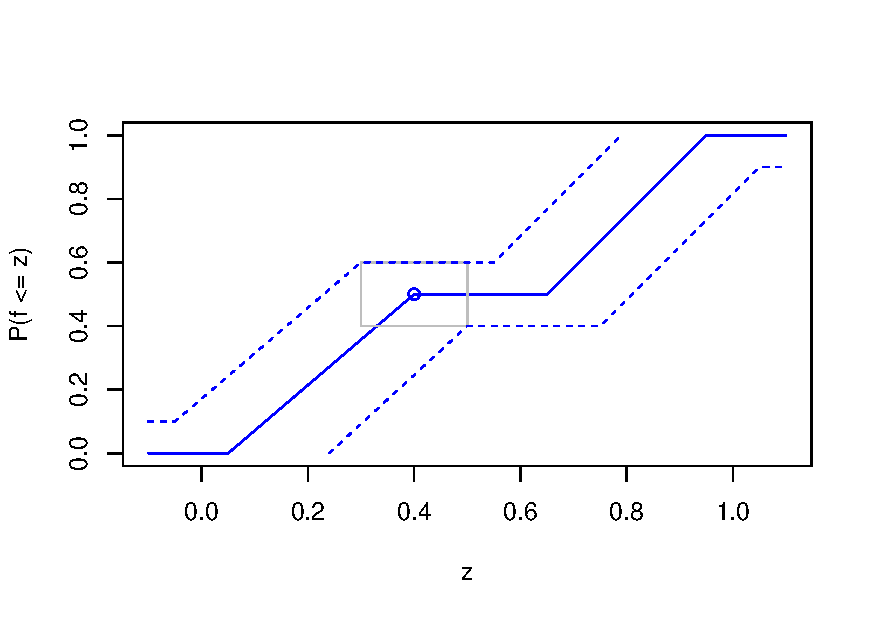
\includegraphics[width=1\linewidth]{Bilder/Levi1}
				%\caption{$R_{L_1,P}(f)$}
				%\label{fig:sub1}
			\end{subfigure}%
			\begin{subfigure}{.5\textwidth}
				\centering
				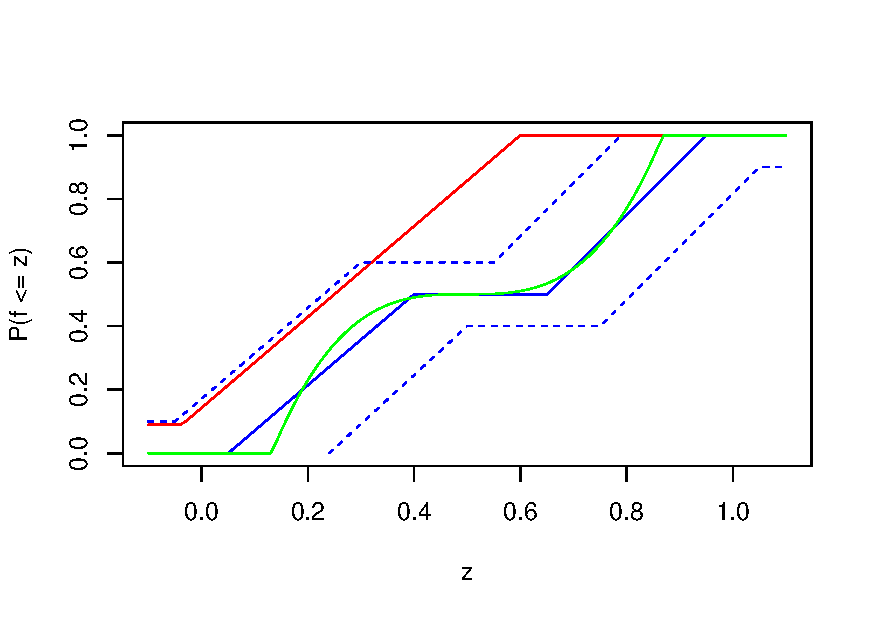
\includegraphics[width=1\linewidth]{Bilder/Levi2}
				%\caption{$R_{l,P}(f)$}
				%\label{$R_{l,P}(f)-R_{l,P}(f^*_P)$}
			\end{subfigure}
			%\caption{Vergleich L1-Loss und Hindge-Loss}
			%\label{fig:test}
		\end{figure}
	\end{frame}
	
	\begin{frame}
		\frametitle{Eigenschaften L\'evi-Abstand}
		\begin{itemize}
			\item $P,P_1,P_2,...$ Verteilungen auf $(E,\mathcal{A})$
			\item $f : E \rightarrow [0,1]$ messbar
		\end{itemize}
		\hfill\break
		Dann gilt:
		\begin{itemize}
			\item $\left| P_1(f) - P_2(f) \right| \leq 4 \, \mathbb{L}_f(P_1,P_2)$
			\item $(f)_*P_m \xrightarrow{m \rightarrow \infty}_{\mathcal{L}} (f)_*P \ \Leftrightarrow \ \mathbb{L}_f(P_m,P) \xrightarrow{m \rightarrow \infty} 0 $
		\end{itemize}
		\hfill\break
		(mehr Eigenschaften \href{https://encyclopediaofmath.org/wiki/Lévy_metric}{\textbf{hier}})
	\end{frame}
	
	
	\section{Haupt-Aussagen}
	
	\begin{frame}
		\frametitle{Satz 3.1 : Abschätzung der Verteilungsfunktionen mit der Rademacherkomplexität}
		\begin{itemize}
			\item $\F \subset \{f : E \rightarrow \R \, \text{ mb.}\}$ gleichmäßig beschränkt
			\item $(\varphi_k)_{k \in \N}$ Familie von Lipschitz-stetigen Funktionen\\
			mit $|\varphi_k(x)-\varphi_k(y)| \leq c_k \, |x-y|$ und $\varphi_k \geq 1_{(-\infty,0]}$
		\end{itemize}
		Dann gilt für jedes $t > 0$, dass
		{\footnotesize
		\begin{align*}
		\mathbb{P} \bigg( &\exists f \in \F : \ P(f \leq 0) > \frac{t}{\sqrt{n}} +  \inf\limits_{k \in \N} \bigg[ \hat{P}_n(\varphi_k \circ f) + 4 c_k \mathcal{RK}_n(\F) + \left( \frac{\log(k)}{n} \right)^{\frac{1}{2}} \bigg] \bigg) \leq 2 e^{-2t^2}
		\end{align*}
		}
		(Beweis-Idee in der Ausarbeitung)
	\end{frame}

	\begin{frame}
		\frametitle{Satz 3.2 : Abschätzung des L\'evy-Abstandes}
		\begin{itemize}
			\item $\F \subset \{f : E \rightarrow [-M,M] \, \text{ mb.}\}$
		\end{itemize}
		dann gilt für jedes $t > 0$, dass
		\begin{align*}
		& \mathbb{P}\left( \sup\limits_{f \in \F} \mathbb{L}_f(P, \hat{P}_n) \geq \frac{t}{\sqrt{n}} + 2\left(\frac{M}{\sqrt{n}} + \mathcal{RK}_n(\F)\right)^{\frac{1}{2}} \right) \leq e^{-2t^2}
		\end{align*}
		(Beweis-Idee in der Ausarbeitung)
	\end{frame}

	\begin{frame}
		\frametitle{Folgerungen}
		Für $\F \subset \{f : E \rightarrow [-M,M] \, \text{ mb.}\}$ gilt:
		\begin{itemize}
			\item $\F$ ist $P$-GC. $\Leftrightarrow \ \sup\limits_{f \in \F} \mathbb{L}_f(P,\hat{P}_n) \xrightarrow{n \rightarrow \infty}_{fs.} 0$
			\item $\F$ ist $P$-Donsker $\Rightarrow \ \exists C>0 \ \forall n \in \N : \ \E\left[ \sup\limits_{f \in \F} \mathbb{L}_f(P,\hat{P}_n) \right] \leq C \, n^{-\frac{1}{4}}$
		\end{itemize}
		(Beweise in der Ausarbeitung)\\
		\hfill\break
		\pause
		Vergleich:\\
		$\F$ ist $P$-Donsker $\Rightarrow \ \exists C>0 \ \forall n \in \N : \ \E\left[ \sup\limits_{f \in \F} |P(f)-\hat{P}_n(f)| \right] \leq C \, n^{-\frac{1}{2}}$\\
		Aussagen über L\'evy-Abstand sind also nicht besonders nützlich für Risiko-Abschätzungen.
	\end{frame}

	\begin{frame}
		\frametitle{Satz 3.5 : Abschätzung mit Margin}
		\begin{itemize}
			\item $P$ Verteilung auf $E \times \{-1,1\}$
			\item $\F \subset \{ f: E \times \{-1,1\} \rightarrow \R \, mb. \}$\\
			(Anschaulich: $f$ ordnet $x$ die Kategorie $y$ zu, falls $f(x,y) > f(x,-y)$)
			\item Margin: $m_f(x,y) := f(x,y) - f(x,-y)$
			\item $RK_n := \mathcal{RK}_n\left( \{f(\cdot,1) \mid f \in \F \} \cup \{f(\cdot,-1) \mid f \in \F \} \right)$
		\end{itemize}
		Dann gilt für jedes $t >0:$ 
		{\small
		\begin{align*}
		\mathbb{P}\vast( \exists & f \in \F : \ P(m_f \leq 0) > \\
		& \inf\limits_{\delta \in (0,1)}\left[ \hat{P}_n(m_f \leq \delta) + \frac{48}{\delta} RK_n + \sqrt{\frac{\log\log_2(\frac{2}{\delta})}{n}} \right] + \frac{t}{\sqrt{n}} \vast) \leq 2 e^{-2t^2}
		\end{align*}
		}
		\hfill\break
		\pause
		$\Rightarrow$ Es lassen sich Aussagen über $R_P(\text{sign}(\Phi(T_n)))$ machen.
	\end{frame}



	\section{Anwendungen}
	
	\begin{frame}
		\frametitle{Anwendungen}
		\begin{itemize}
			\item Artikel findet Zusammenhang zwischen L\'evi-Abstand und Rademacher-Komplexität
			\item (Bem. 4.2) $\mathcal{RK}_n(\F) = \mathcal{RK}_n(co(\F)) \ \Rightarrow$ interessant für z.B. 'Boosting'-Algorithmen
			\item Klassifikatoren $\text{sign}\circ\Phi(T_n)$ um Entscheidungsgrenze herum instabil, Artikel liefert Methoden damit umzugehen.
		\end{itemize}
	\end{frame}



	\section{Vergleich}
	
	\begin{frame}
		\frametitle{Satz 5.1 : Donsker-Klassen und RKHS}
		\begin{itemize}
			\item $P$ Verteilung auf $[0,1] \times \{-1,1\}$
			\item $H_\sigma$ RKHS zu $K_\sigma(x,y) = e^{-\frac{(x-y)^2}{\sigma^2}}$
			\item $(f_\alpha)_{\alpha \in \Lambda_{r,\sigma}} = \F_{r,\sigma} := \{f \in H_{\sigma} \mid r \geq ||f||_{H_{\sigma}} \}$
			\item Verlustfunktion $L: \R \times \{-1,1\}$ im 1. Arg. Lipschitz-stetig
			\item ERM $\Phi_{r,\sigma} := \arg\min\limits_{f \in \F_{r,\sigma}} R_{L,\hat{P}_n}(f)$
		\end{itemize}
		Dann gilt:
		\begin{align*}
		\exists C_1,&C_2>0 \ \forall n \in \N \ \forall r,\sigma > 0 : \\
		& \E \left[ R_{L,P}(\Phi_{r,\sigma}(T_n)) - \inf\limits_{\alpha \in \Lambda_{r,\sigma}} R_{L,P}(f_\alpha) \right] \leq \frac{r}{\sigma} \frac{C_1}{\sqrt{n}} + \frac{C_2}{\sqrt{n}}
		\end{align*}
	\end{frame}

	\begin{frame}
		\frametitle{Satz 5.1 : Donsker-Klassen und RKHS (Beweis-Idee)}
		Letzter Vortrag: $\forall f \in H_\sigma : \ ||f||_{TV} \leq \sqrt{\frac{2}{\sigma^2}} ||f||_{H_\sigma}$\\
		$\Rightarrow \ \forall f \in \F_{r,\sigma} : \ ||f||_{TV} \leq \sqrt{\frac{2}{\sigma^2}} r$\\
		$\Rightarrow \ \F_{r,\sigma} \subset E_{\frac{r}{\sigma}\sqrt{2}} := \{f : [0,1] \rightarrow \R \mid \frac{r}{\sigma}\sqrt{2} \geq ||f||_{TV} \}$\\
		$\overset{L\text{ Lipschitz}}{\Rightarrow} \ \frac{\sigma}{r} L(\F_{r,\sigma},-1) \cup \frac{\sigma}{r}L(\F_{r,\sigma},1) \subset E_{C}$\\
		\hfill\break
		\pause
		\cite{DudleyUCLT} Seite 329 $\ \Rightarrow \ E_{C}$ ist uniform Donsker.\\
		$\Rightarrow \ \frac{\sigma}{r} L(\F_{r,\sigma},i)$ sind $P_i:=P_{X\mid Y=i}\,$-Donsker\\
		$\Rightarrow \ \exists c >0 : \ \E\left[ \sup\limits_{f \in \F_{r,\sigma}} \left|P_i\left(\frac{\sigma}{r}L\left(f(X),i\right)\right)-\widehat{(P_i)}_{n}\left(\frac{\sigma}{r}L\left(f(X),i\right)\right) \right| \right] \leq \frac{c}{\sqrt{n}}$\\
		(Trick mit Bedingung auf $Y$ aus Lemma 1.4)\\
		$\Rightarrow \ \E\left[ \sup\limits_{f \in \F_{r,\sigma}} \left|R_{L,P}(f)-\inf\limits_{g \in  \F_{r,\sigma}} R_{L,P}(g) \right| \right] \leq \frac{r}{\sigma} \frac{C_1}{\sqrt{n}} + \frac{C_2}{\sqrt{n}} \ \ \ \ \ \ \ \  \qed$
	\end{frame}
	
	\begin{frame}
		\frametitle{Satz 5.2 : RKHS. Familien-Risiko}
		\begin{itemize}
			\item $P$ Verteilung auf $[0,1] \times \{-1,1\}$
			\item $\F_{r,\sigma} := \{f \in H_{\sigma} \mid r \geq ||f||_{H_{\sigma}} \}$
			\item Verlustfunktion $l$ Hinge-Loss
			\item $P$ hat GNE $\alpha \in (0,\infty)$
		\end{itemize}
		Dann gilt:
		\begin{align*}
		\exists c,&C_\alpha>0 \ \forall n \in \N \ \forall r,\sigma > 0 : \\
		& \inf_{f \in \F_{r,\sigma}} R_{l,P}(f) - \inf_{f:[0,1] \rightarrow \{-1,1\}}R_{l,P}(f) \leq c\left(\frac{1}{\sigma r^2} + C_\alpha 2^{\frac{\alpha}{2}} \sigma^{\alpha}\right)
		\end{align*}
		($C_\alpha$ wie in der Definition des GNE aus dem letzten Vortrag)\\
		(Direkte Folgerung aus Thm. 2.7 in \cite{St1})
	\end{frame}

	\begin{frame}
		\frametitle{Bemerkung 5.4 : ERM in größer werdenden Familien}
		Wähle $\sigma_n$, $r_n$, sodass $\E\left[ R_{l,P}(\Phi_{r_n,\sigma_n}) - \inf\limits_{f:[0,1] \rightarrow \{-1,1\}} R_{l,P}(f) \right] \searrow 0$
		\begin{itemize}
			\item 5.1 $\Rightarrow \ \E \left[ R_{l,P}(\Phi_{r_n,\sigma_n}(T_n)) - \inf\limits_{f \in \F_{r_n,\sigma_n}} R_{l,P}(f) \right] \leq \frac{r_n}{\sigma_n} \frac{c}{\sqrt{n}} + \frac{c}{\sqrt{n}}$
			\item 5.2 $\Rightarrow \ \inf_{f \in \F_{r_n,\sigma_n}} R_{l,P}(f) - \inf_{f:[0,1] \rightarrow \{-1,1\}}R_{l,P}(f) \leq \frac{c}{\sigma_n r_n^2} + c \sigma_n^{\alpha}$
		\end{itemize}
		\pause
		$\Rightarrow \ \E\left[ R_{l,P}(\Phi_{\lambda_n,\sigma_n}) - \inf\limits_{f:[0,1] \rightarrow \{-1,1\}} R_{l,P}(f) \right] \leq c\, \max\left( \frac{1}{\sigma_n r_n^2} , \sigma_n^\alpha , \frac{r_n}{\sigma_n \sqrt{n}} , \frac{1}{\sqrt{n}} \right)$
		Wähle $\sigma_n = n^{-\frac{1}{3(\alpha+1)}}$ und $r_n = n^{\frac{1}{6}}$\\
		$\Rightarrow \ \E\left[ R_{l,P}(\Phi_{r_n,\sigma_n}) - \inf\limits_{f:[0,1] \rightarrow \{-1,1\}} R_{l,P}(f) \right] \leq c\, n^{-\frac{\alpha}{3(\alpha+1)}}$
	\end{frame}

	\begin{frame}
		\frametitle{Satz 5.5 : KDE mit Margin-Abschätzung}
		\begin{itemize}
			\item $P$ Verteilung auf $[0,1]\times \{-1,1\}$
			\item $P$ habe TNE $q \in [0,\infty]$
			\item Voraussetzung: $\exists \varepsilon > 0 : \ \left| \int_\R \int_\R (p_y(x) - p_y(x+t\sigma)) \frac{e^{-t^2}}{\sqrt{2\pi}} \, dt \, dP_y(x) \right| \leq c\, \sigma^{\varepsilon}$
			\item $\sigma_n = n^{-\frac{1}{2(1+\varepsilon)}}$
			\item $\Phi^N_n(x) := \Phi^{Naiv}(T_n)(x) = \frac{1}{n} \sum\limits_{i=1}^n Y_i \frac{K_{\sigma_n}(x,X_i)}{\sqrt{2\pi\sigma^2}}$
			
		\end{itemize}
		\pause
		Dann $\exists C > 0 \ \forall n \in \N :$
		\begin{align*}
		& \E\left[ R_P(\text{sign}(\Phi_n^N)) - \inf_{f:[0,1] \rightarrow \{-1,1\}} R_P(f) \right] \leq C\, n^{-\frac{\varepsilon q}{2(q+1)(1+\varepsilon)}}
		\end{align*}
		(Beweis in der Ausarbeitung, verwende 3.5)
	\end{frame}

	\begin{frame}
		\frametitle{Satz 5.6 : ERMR mit Margin-Abschätzung}
		\begin{itemize}
			\item $P$ Verteilung auf $[0,1]\times \{-1,1\}$
			\item $P$ habe GNE $\alpha \in (0,\infty)$
			\item $\lambda_n = n^{-\frac{1}{3}}$ und $\sigma_n = n^{-\frac{1}{3(\alpha+1)}}$
			\item ERMR $\Phi_{\lambda_n, \sigma_n}(T_n) = \arg \min\limits_{f \in H_{\sigma_n}} \left( \lambda_n ||f||_{H_{\sigma_n}}^2 + R_{L,\hat{P}_n}(f) \right)$\\
			letzter Vortrag $\Rightarrow \ \Phi_{\lambda_n, \sigma_n}(T_n)(x) = \sum\limits_{i=1}^n \alpha^n_i Y_i K_{\sigma_n}(x,X_i)$
			\item Voraussetzung: $\exists \varepsilon \in [0,\frac{1}{2}) : \ \E\left[\sum\limits_{j=1}^n \alpha^n_j\right] = \mathcal{O}(n^{\varepsilon})$
		\end{itemize}
		\pause
		Dann $\exists C > 0 \ \forall n \in \N :$
		\begin{align*}
		& \E\left[ R_P(\text{sign}(\Phi_{\lambda_n, \sigma_n}(T_n))) - \inf_{f:[0,1] \rightarrow \{-1,1\}} R_P(f) \right] \leq C\, n^{-\min\left(\frac{1-2\varepsilon}{4}, \frac{\alpha}{3(\alpha+1)}\right)}
		\end{align*}
		(Beweis in der Ausarbeitung, verwende 3.5)
	\end{frame}
	
	\begin{frame}
		\frametitle{Quellen und Verweise}
		\begin{bibdiv}
			\begin{biblist}
				
				\bib{KP1}{article}{
					author={Koltchinskii, V.},
					author={Panchenko, D.},
					title={Empirical margin distributions and bounding the generalization
						error of combined classifiers},
					journal={Ann. Statist.},
					volume={30},
					date={2002},
					number={1},
					pages={1--50},
					issn={0090-5364},
					doi={10.1214/aos/1015362182},
				}
			
				\bib{St1}{article}{
					author={Steinwart, Ingo},
					author={Scovel, Clint},
					title={Fast rates for support vector machines using Gaussian kernels},
					journal={Ann. Statist.},
					volume={35},
					date={2007},
					number={2},
					pages={575--607},
					issn={0090-5364},
					doi={10.1214/009053606000001226},
				}
				
				\bib{DudleyUCLT}{book}{
					author={Dudley, R. M.},
					title={Uniform central limit theorems},
					series={Cambridge Studies in Advanced Mathematics},
					volume={142},
					edition={2},
					publisher={Cambridge University Press, New York},
					date={2014},
					pages={xii+472},
					isbn={978-0-521-73841-5},
					isbn={978-0-521-49884-5},
				}
				
				\bib{VaartWCEP}{book}{
					author={van der Vaart, Aad W.},
					author={Wellner, Jon A.},
					title={Weak convergence and empirical processes},
					series={Springer Series in Statistics},
					note={With applications to statistics},
					publisher={Springer-Verlag, New York},
					date={1996},
					pages={xvi+508},
					isbn={0-387-94640-3},
					doi={10.1007/978-1-4757-2545-2},
				}
				
			\end{biblist}
		\end{bibdiv}
		\hfill\break
		\centering
		Vielen Dank für Ihre Aufmerksamkeit!
	\end{frame}
	
\end{document}
